%
% File acl2017.tex
%
%% Based on the style files for ACL-2015, with some improvements
%%  taken from the NAACL-2016 style
%% Based on the style files for ACL-2014, which were, in turn,
%% based on ACL-2013, ACL-2012, ACL-2011, ACL-2010, ACL-IJCNLP-2009,
%% EACL-2009, IJCNLP-2008...
%% Based on the style files for EACL 2006 by 
%%e.agirre@ehu.es or Sergi.Balari@uab.es
%% and that of ACL 08 by Joakim Nivre and Noah Smith

\documentclass[11pt,a4paper]{article}
\usepackage[hyperref]{acl2017}
\usepackage{times}
\usepackage{latexsym}
\usepackage{graphicx}
\usepackage{booktabs}
\usepackage{amsmath}
\usepackage{todonotes}
\usepackage{multirow}
\usepackage{enumitem}
\usepackage{amsfonts}
\usepackage{url}

\makeatletter
\newcommand{\@emptybiblabel}[1]{}
\makeatother
\DeclareMathOperator*{\argmax}{arg\,max}
\setlength\titlebox{3.5cm}    % Expanding the titlebox

\newcommand*{\checktikz}[1][]{\tikz[x=1em, y=1em]\fill[#1] (0,.35) -- (.25,0) -- (1,.7) -- (.25,.15) -- cycle;}
\newcommand*{\crosstikz}[1][]{\tikz[x=1em, y=1em]\fill[#1] (0,0) -- (1,1) -- (0.5,0.5) -- (0.1,0.1) -- cycle;}

\newcommand\BibTeX{B{\sc ib}\TeX}
\newcommand{\Correct}{\checktikz[draw=black]}
\newcommand{\ValidMiss}{\checktikz[draw=gray,fill=white]}
\newcommand{\Valid}{\checktikz[draw=gray,fill=white]}
\newcommand{\Missed}{\checktikz[draw=black]} %\textsf{X}~}
\newcommand{\Wrong}{} %\textsf{X}~}

\newcommand{\U}{\mathbb{U}}

\title{Are you asking the right questions? \\ Automatically Generating Clarification Questions}

\date{}

\begin{document}
\maketitle
\begin{abstract}
	
Inquiry is fundamental to communication, and machines cannot effectively collaborate with humans unless they can ask questions. The goal of this thesis work is to explore how can a machine automatically generate clarification questions when faced with uncertainty, a goal of increasing importance in today's automated society. We do a preliminary study using data from StackExchange, a plentiful online resource where people routinely ask clarifying questions to posts so that they can better offer assistance to the original poster. We build neural network models inspired by the idea of the expected value of perfect information: a good question is one whose expected answer is going to be most useful.
To build generalizable systems, we propose two research directions: a template based model and a sequence-to-sequence based neural generative model.
\end{abstract}

\section{Introduction}\label{introduction}

A main goal of asking questions is to fill information gaps, typically through clarification questions, which naturally occur in conversations. 
A good question is one whose \emph{likely answer} is going to be the most useful.
Consider the exchange in Figure~\ref{askubuntu_post}, in which an initial poster (who we'll call ``Terry'') asks for help configuring environment variables.
This question is underspecified and a responder (``Parker'') asks a clarifying question ``\textsf{\small (a) What version of Ubuntu do you have?}''
Parker could alternatively have asked one of:

\textsf{\small(b) Is the moon waxing or waning?}

\textsf{\small(c) Are you running Ubuntu 14.10 kernel 4.4.0-59-generic on an x86\_64 architecture?}

\noindent
Parker should not ask (b) because it's not useful; they should not ask (c) because it's too specific and an answer of ``No'' gives little help.
Parker's question (a) is optimal: it is both likely to be useful, and is plausibly answerable by Terry.
Our goal in this work is to automate Parker.
Specifically, after Terry writes their initial post, we aim to generate a clarification question so that Terry can immediately amend their post in hopes of getting faster and better replies.
\begin{figure}[!t]
	\centering
	\setlength\fboxsep{1pt}
	\setlength\fboxrule{0.5pt}
	\fbox{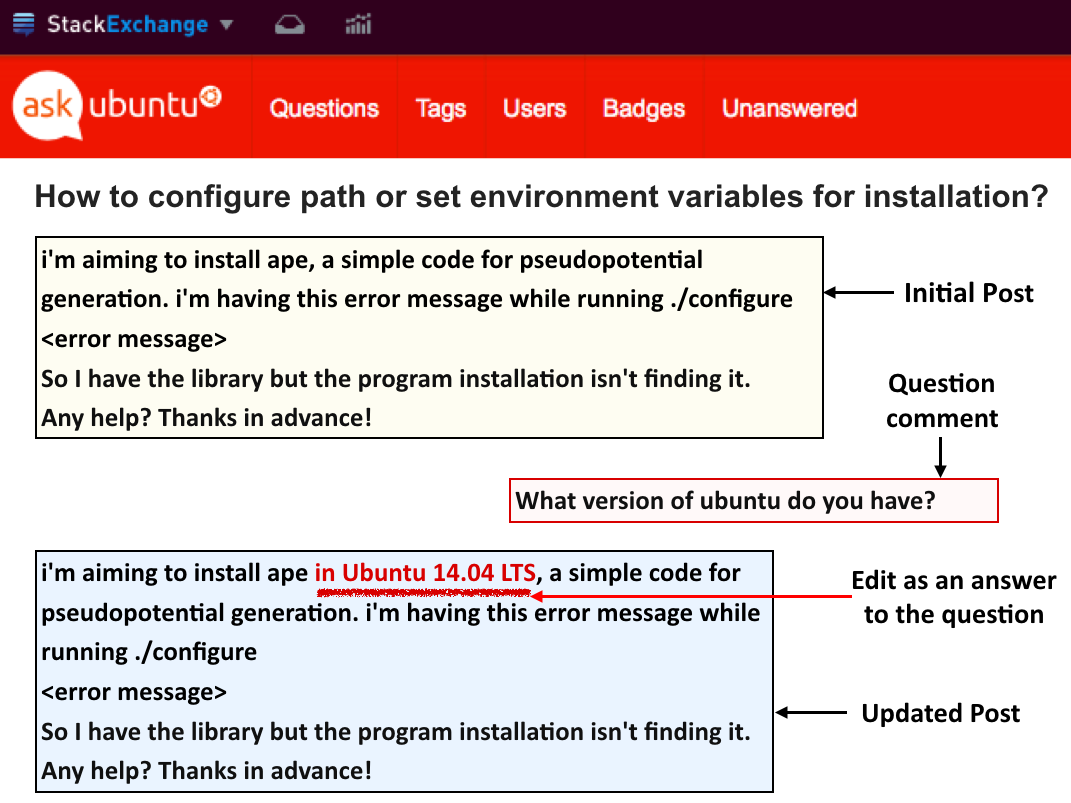
\includegraphics[width=0.47\textwidth]{askubuntu_post}}
	\caption{A post on an online Q \& A forum ``askubuntu.com'' is updated to fill the missing information pointed out by the question comment}
	%\vspace{-1.0em}
	\label{askubuntu_post}
\end{figure}
%

Our work has two main contributions: 
\begin{enumerate}[noitemsep,nolistsep]
%\item Identifying the problem of generating clarification questions as a problem worth of study, both in its own right and as part of the larger problem of building naturalistic conversational systems. 
\item A novel neural-network model for addressing this task that integrates the notion of expected value of perfect information (\S\ref{model}). % , a classic formalization from AI
\item A novel dataset, derived from StackExchange, that enables us to learn a model to ask clarifying questions by looking at the types of questions people ask (\S\ref{dataset_creation}).\footnote{We use data from StackExchange; per license cc-by-sa 3.0, the data is ``intended to be shared and remixed'' (with attribution). We will release all of the data we extract.}
\end{enumerate}

To develop our model we take inspiration from the decision theoretic framework of the Expected Value of Perfect Information (EVPI), a measure of the value of gathering additional information. In our setting, we use EVPI to calculate which question is most likely to elicit an answer that would make the post more informative.
Formally, for an input post $p$, we want to choose a question $q$ that maximizes $\mathbb{E}_{a \sim p,q}[\U(p+a)]$, where $a$ is a hypothetical answer and $U$ is a utility function measuring the \emph{completeness} of post $p$ if $a$ were to be added to it.
To achieve this, we construct two models:
(1) an answer model, which estimates $\mathbb{P}[a~|~p,q]$, the likelihood of receiving answer $a$ if one were to ask question $q$ on post $p$;
(2) a completeness model, $\U(p)$, which measures how complete a post is.
Given these two models, at prediction time we search over a shortlist of possible questions for that which maximizes the EVPI.

We are able to train these models jointly based on $(p,q,a)$ triples that we extract automatically from StackExchange.
Figure~\ref{askubuntu_post} depicts how we do this using StackExchange's edit history.  In the figure, the initial post fails to state what version of Ubuntu is being run. In response to Parker's question in the comments section, Terry, the author of the post, edits the post to answer Parker's clarification question. We extract the initial post as $p$, question posted in the comments section as $q$, and edit to the original post as answer $a$ to form our $(p,q,a)$ triples. 

Our results show significant improvements from using the EVPI formalism over both standard feedforward network architectures and bag-of-ngrams baselines, even when our system builds on strong information retrieval scaffolding. In comparison, without this scaffolding, the bag-of-ngrams model outperforms the feedforward network. We additionally analyze the difficulty of this task for non-expert humans. 

\begin{figure*}[t]
	\centering
	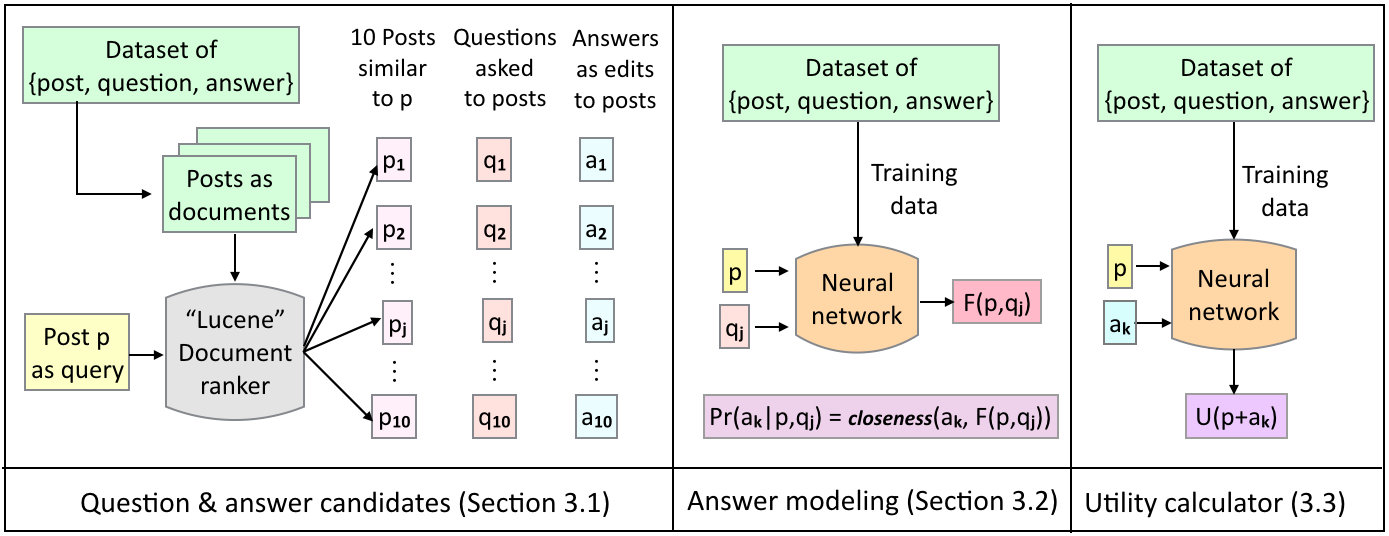
\includegraphics[width=0.85\textwidth]{model}
	\caption{ The behavior of our model during test time. Given a post $p$, we retrieve 10 posts similar to $p$ using Lucene and consider the questions asked to those as question candidates and the edits made to the posts in response to the questions as answer candidates. Our answer model generates an answer representation $F(p,q_j)$ for each question candidate $q_j$ and calculates how close is an answer candidate $a_k$ to $F(p,q_j)$. Our utility calculator calculates the utility of the post if it were updated with the answer $a_k$. We select the question $q_j$ that maximizes the expected utility of the post $p$ (Equation~\ref{evpi_equation}).}
	\label{model}
	\vspace{-0.5em}
\end{figure*}

\section{Related Work} \label{related_work}

The problem of question generation has received sparse attention from the natural language processing community. Most prior work focuses on generating reading comprehension questions:  given text, write questions that one might find on a standardized test \cite{vanderwende2008importance,heilman2011automatic,rus2011question,olney2012question}.  Comprehension questions, by definition, are answerable from the provided text. Clarification questions are not.  

%Outside reading comprehension questions, \newcite{labutov2015deep} generate high-level question templates by crowdsourcing and given a text segment, rank question templates that are relevant. However the crowdsourcing method of collecting data leads to significantly less data than we collect using our method. \newcite{liu2010automatic} use template question generation to help authors write better related work sections. \newcite{mostafazadeh2016generating} introduce a Visual Question Generation task where they consider question generation from images, a multi-modal variant of question generation. 
%\newcite{penas2010filling} identify the notion of missing information similar to us but they attempt to fill the knowledge gaps in a text with the help of external knowledge bases, whereas we instead ask clarification questions. \newcite{artzi2011bootstrapping} use human-generated clarification questions to drive a semantic parser where the clarification questions are aimed towards simplifying a user query; whereas we generate clarification questions aimed at  identifying missing information in a text. 

Outside reading comprehension questions, \newcite{labutov2015deep} studied the problem of generating question templates via crowdsourcing, \newcite{liu2010automatic} use template based question generation to help authors write better related work sections, \newcite{mostafazadeh2016generating} consider question generation from images, and  \newcite{artzi2011bootstrapping} use human-generated clarification questions to drive a semantic parser.

\section{Model Description}\label{model}

In order to choose what question to ask, we build a neural network model inspired by the theory of expected value of perfect information (EVPI). EVPI is a measurement of: if I were to acquire information X, how useful would that be to me? However, because we haven't acquired X yet, we have to take this quantity in expectation over all possible X, weighted by each X's likelihood. In the question generation setting, for any given question $q$ that we can ask, there is set $A$ of possible answers that could be given. For each possible answer $a \in A$, there is some probability of getting that answer, and some utility if that were the answer we got. The value of this question $q$ is the expected utility, over all possible answers. The theory of EVPI then states that we want to choose the question $q$ that maximizes:
\begin{equation}\label{evpi_equation}
\argmax_{q \in Q} \sum_{a \in A} \mathbb{P}[a | p,q] \U(p+a)
\end{equation} 

In Eq~\ref{evpi_equation}, $p$ is the post, $q$ is a potential question from a set of candidate questions $Q$ (\S\ref{question_candidate_generator}) and $a$ is a potential answer from a set of candidate answers $A$ (\S\ref{question_candidate_generator}). $\mathbb{P}[a | p,q]$ (\S\ref{answer_modeling}) measures the probability of getting an answer $a$ given an initial post $p$ and a clarifying question $q$. $\U(p+a)$ (\S\ref{utility_calculator}) measures how useful it would be if $p$ were augmented with answer $a$. Finally, using these pieces, we build a joint neural network that we can optimize end-to-end over our data (\S\ref{neural_network}). Figure~\ref{model} describes the behavior of our model during test time. 

\subsection{Question \& Answer Candidate Generator}\label{question_candidate_generator}

Given a post, our first step is to generate a set of candidate questions and answers. One way that humans learn to ask questions is by looking at how others ask questions in a similar situation. Using this intuition, we first identify 10 posts similar to the given post in our dataset using Lucene\footnote{\url{https://lucene.apache.org/}} (a software extensively used in information retrieval) and then consider the questions asked to these posts as our set of question candidates and the edits made to the posts in response to the questions as our set of answer candidates.

\subsection{Answer Modeling}\label{answer_modeling}

Given a post $p$ and a question candidate $q_i$, our second step is to calculate how likely is this question to be answered using one of our answer candidates $a_k$. To calculate this probability, we first generate an answer representation $F(p,q_i)$ and then measure how close is the answer candidate $a_k$ to our answer representation using the equation:
\begin{align}
\mathbb{P}[a_k |p,q_i]  
&= \frac 1 Z \exp\left[- \lambda || a_k  -  F(p,q_i) ||^2\right]
\end{align}
where $\lambda$ is a tunable parameter that controls the variance of the distribution. 

We train our answer generator using the following intuition: a question can be asked in several different ways. For e.g. in Figure~\ref{askubuntu_post}, the question ``\textsf{\small What version of Ubuntu do you have?}'' can be asked in other ways like ``\textsf{\small What version of operating system are you using?}'', ``\textsf{\small Version of OS?}", etc.  
Additionally, a question can generate several different answers. For instance, ``\textsf{\small Ubuntu 14.04 LTS}", ``\textsf{\small Ubuntu 12.0}", ``\textsf{\small Ubuntu 9.0}", are all valid answers. To capture these generalizations, we define the following loss function:
\begin{align}\label{eq_answer_generator}
\textrm{loss}_{\textrm{ans}}(\bar p, \bar q, \bar a, Q) 
&=  {|| F(\bar p, \bar q) - \bar a||}^2 & \\
&\hspace{-25mm} +  \sum_{j \in Q} \Big ( {|| F(\bar p, \bar q) - \bar{a_j} ||}^2  (1 - \tanh{(|| \bar q - \bar{q_j} ||^2)}) \Big ) &\nonumber
\end{align}
%
 In equation~\ref{eq_answer_generator}, the first term forces the answer representation $F(\bar p_i, \bar q_i)$ to be as close as possible to the correct answer $a_i$ and the second term forces it to be close to the answer $a_j$ corresponding to a question $q_j$ very similar to $q_i$ (i.e. $||\bar{q_i} - \bar{q_j}||$ is near zero).

\begin{table*}[t]
	\small
	\centering
	\begin{tabular}{l|cccc|cccc}
		\toprule
		& \multicolumn{4}{c|}{\textbf{Lucene negative candidates}} & \multicolumn{4}{c}{\textbf{Random negative candidates}} \\
		\textbf{Models} & Acc & MRR & R@3 & R@5 & Acc & MRR & R@3 & R@5\\
		\midrule
		Random  & 10.0 & 29.3 & 30.0 & 50.0 &10.0 & 29.3 & 30.0 & 50.0 \\
		Bag-of-ngrams & 11.6 & 31.3 & 32.5 & 54.6 & 54.9 & 70.5 & 83.1 & 92.0 \\
		Feed-forward & 17.4 & 37.8 & 43.2 & 63.9 &  49.0 & 66.8 & 81.3 & 92.8 \\
		EVPI & \bf 23.3 & \bf 43.4 & \bf 51.0 & \bf 70.3 & \bf 61.1 & \bf 75.5 & \bf 87.9  & \bf 95.8  \\
		\bottomrule
	\end{tabular}
	\caption{Results of two setups `Lucene negative candidates' and `Random negative candidates' on askubuntu when trained on a combination of three domains: askubuntu, unix and superuser.  We report four metrics: accuracy (percent of time the top ranked question was correct),
		mean reciprocal rank (the reciprocal of the ranked position of the correct question in the top 10 list), recall at 3 (percent of time the correct answer is in the top three) and
		recall at 5.}
	\label{tab:results_topN}
	\vspace{-1.0em}
\end{table*}

\subsection{Utility Calculator}\label{utility_calculator}
Given a post $p$ and an answer candidate $a_k$, our third step is to calculate the utility of the updated post i.e. $\U(p + a_k)$ which measures how useful it would be if a given post $p$ were augmented with an answer $a_k$. We use the intuition that a post $p_i$, when updated with the answer $a_i$ that it is paired with in our dataset, would be more complete than if it is updated with some other answer $a_j$. Therefore we label all the $(p_i, a_i)$ pairs from our dataset as positive and label $p_i$ paired with other nine answer candidates generated using Lucene (\S\ref{question_candidate_generator}) as negative.  The utility of the updated post is then defined as $\U(p+a) = \sigma ( F(\bar{p}, \bar{a}) )$ where $F$ is a feedforward neural network. We want this utility to be close to one for all the positively labelled $(p,a)$ pairs and close to zero for all the negatively labelled $(p, a)$ pairs. We therefore define our loss using the binary cross-entropy formulation below:
\begin{align}\label{eq_utility_calculator}
\textrm{loss}_{\textrm{util}}(y, \bar p, \bar a) &= y \log(\sigma (F(\bar{p}, \bar{a})))
\end{align}

\subsection{Our joint neural network model}\label{neural_network}
Our fundamental representation is based on recurrent neural network, specifically long short-term memory architecture (LSTM) \cite{hochreiter1997long} over word embeddings obtained using a GloVe \cite{pennington2014glove} model trained on the entire datadump of StackExchange. We define three LSTMs corresponding to $p$, $q$ and $a$ and two feedforward neural networks corresponding to our answer model $F(\bar{p},\bar{q})$ and our utility calculator $F(\bar{p}, \bar{a})$. We jointly train the parameters of all our neural network models to minimize the sum of the loss of our answer model (Eq~\ref{eq_answer_generator}) and our utility calculator (Eq~\ref{eq_utility_calculator}):
%
\begin{align}
\sum_i \textrm{loss}_{\textrm{ans}}(\bar p_i, \bar q_i, \bar a_i, Q_i)  
+  \textrm{loss}_{\textrm{util}}(y_i, \bar p_i, \bar a_i)
\end{align}
%
Given such an estimate $\mathbb{P}[a|p,q]$ of an answer and a utility $\U(p+a)$ of the updated post, predictions can be done by choosing that ``$q$'' that maximizes Eq~\ref{evpi_equation}. 

\section{Experiments and Results}

\subsection{Dataset}\label{dataset_creation}
StackExchange is a network of online question answering websites containing timestamped information about the posts, comments on the post and the history of the revisions made to the post. Using this, we create our dataset of \{\textit{post, question, answer}\} triples: where \textit{post} is the initial unedited post, \textit{question} is the comment containing a question and \textit{answer} is the edit made to the post that matches the question comment. We extract a total of 37K triples from the following three domains of StackExchange: askubuntu, unix and superuser.

\subsection{Experimental Setups}\label{task_setup}
We define our task as given a post and 10 question candidates, select the correct question candidate. For every post $p$ in our dataset of $(p, q, a)$ triples, the question $q$ paired with $p$ is our positive question candidate. We define two approaches to generate negative question candidates: \\
\textbf{Lucene Negative Candidates}: We retrieve nine question candidates using Lucene (\S\ref{question_candidate_generator}) and \\
\textbf{Random Negative Candidates}: We randomly sample nine other questions from our dataset.

\subsection{Primary Research Questions}\label{experiments_results}
Our primary research questions that we evaluate experimentally are:\\
a. Does a neural architecture improve upon a simple bag-of-ngrams baseline?\\
b. Does the EVPI formalism provide leverage over a similarly expressive feed-forward network?\\\
c. How much harder is the task when the negative candidate questions come from Lucene rather than selected randomly?
%\begin{enumerate}[noitemsep,nolistsep]
%	\item Does a neural architecture improve upon a simple bag-of-ngrams baseline?
%	\item Does the EVPI formalism provide leverage over a similarly expressive feed-forward network?
%	\item How much harder is the task when the negative candidate questions come from Lucene rather than selected randomly?
%\end{enumerate}

\subsection{Baseline Methods}\label{baselines}

\textbf{Random}: Randomly permute the set of 10 candidate questions uniformly.\\
\textbf{Bag-of-ngrams}: Construct a bag-of-ngrams representation for the post, the question and the answer and train a classifier to minimize hinge loss on misclassification loss. \\
\textbf{Feed-forward neural}: Concatenate the post LSTM representation, the question LSTM representation and the answer LSTM representation and feed it through a feed forward neural network of two fully-connected hidden layers.

\subsection{Results}

We describe results on a test split of askubuntu when our models are trained on the union of all data, summarized in Table~\ref{tab:results_topN}. The left half of this table shows results when the candidate sets is from Lucene---the ``hard'' setting and the right half of this table shows the same results when the candidate set is chosen randomly---the ``easy'' setting. Here, we see that for all the evaluation metrics, EVPI outperforms all the baselines by at least a few percentage points. A final performance of 51\% recall at 3 in the ``hard'' setting is encouraging, though clearly there is a long way to go for a perfect system. 

\section{How good are humans at this task?}

In this section we address two natural questions:
(a) How does the performance of our system compare to a human solving the same task?
(b) Just because the system selects a question that is not the exact gold standard question, is it certainly wrong?
To answer these questions, we had 14 computer science graduate students perform the task on $50$ examples.
Most of these graduate students are \emph{not} experts in unix or ubuntu, but are knowledgable.
Given a post and a randomized list of ten possible questions, they were instructed to select what they thought was the \emph{single} best question to ask, and additionally mark as ``valid'' any additional questions that they thought would also be okay to ask.
We also asked them to rate their confidence in $\{0,1,2,3\}$.
Most found this task quite challenging because many of the questions are about subtle nuances of operating system behavior.

These annotator's accuracy on the ``hard'' task of Lucene-selected questions, was only 36\%, significantly better than our best system (23\%), but still far from perfect.
If we limited to those examples on which they were more confident (confidence of 2 or 3), their accuracy raised to 42\%, but never surpassed that.
A major problem for the human annotators is the amount of background knowledge required to solve this problem.
On an easier domain, or with annotators who are truly experts, we might expect these numbers to be higher.

\section{Proposed Research Directions}

In our preliminary work, we focus on the question selection problem i.e. select the right clarification question from a set of prior questions.
To enable our system to generalize well to new context, we propose two new research directions:
%To make the system more general, it needs to generalize to new context well. Towards this goal, we propose two new research directions:

\subsection{Template Based Question Generation}

 Consider a template like ``What version of \_\_\_  are you running?''. This template can generate thousands of specific variants found in the data like ``What version of Ubuntu are you running?'',  ``What version of apt-get are you running?'', etc. We propose the following four step approach to our template based question generation method:

\begin{enumerate}[noitemsep,nolistsep] 
\item Cluster questions based on their lexical and semantic similarity. % from a huge collection of questions.
\item Generate a template for each cluster by removing topic specific words from questions.
\item Given a post, select a question template from a set of candidate question templates using a model similar to our preliminary work.
\item Finally, fill in the blanks in the template using topic specific words retrieved from the post. 
\end{enumerate}

\subsection{Neural Network Generative Model}
  
Sequence-to-sequence neural network models have proven to be effective for several language generation tasks like machine translation \cite{sutskever2014sequence}, dialog generation \cite{serban2016building}, etc. These models are based on an encoder-decoder framework where the encoder takes in a sequence of words and generates a vector representation of the input. The decoder then takes in this input representation and generates a sequence of words as its output. 

On similar lines, we propose a model for generating the clarification question one word at a time, given the words of a post. A recent neural generative question answering model \cite{yin2015neural} built an answer language model which decides, at each time step, whether to generate a common vocabulary word or an answer word retrieved from a knowledge base. %Thus the model is built on an encoder-decoder framework equipped with the ability to enquire a knowledge base of facts contained in the form of entity-relationship triples. 
Inspired from this work, we propose to build a question generation model which will decide, at each time step, whether to generate a common vocabulary word or a topic specific word retrieved from the current post, thus incorporating the template based method into a more general neural network framework.

\section{Conclusion}

In our work we describe a new dataset for question generation, and build a model that integrates state-of-the-art neural network structure with the classic notion of expected value of perfect information, which effectively models a pragmatic choice on the part of the questioner: how do I \emph{imagine} the other party would answer if I were to ask this question. Such pragmatic priciples have recently been shown to be useful in other tasks as well \cite{golland2010game,smith2013learning,orita2015discourse,andreas2016reasoning}.

One main avenue for improvement of this work is in evaluation: given that this task is so difficult for humans, but also given that there is no single right question to ask, how can we better measure performance at this task? This is exactly the same question faced in much research in dialog and generation more broadly \cite{paek2001empirical,lowe2015ubuntu,liu2016not,kannan2017adversarial}. Finally, asking question is a natural component of dialog, and building a collaborative dialog system that can naturally converse with a user is a broad long term goal.

\bibliography{question_generation}
\bibliographystyle{acl_natbib}

\end{document}
